\documentclass[12pt,aspectratio=169]{beamer}

\usepackage[T1]{fontenc}
\usepackage[spanish,es-nodecimaldot]{babel}
\usepackage{lmodern}
\usepackage{textcomp}
\usepackage{amsmath,amssymb}
\usepackage{graphicx}
\usepackage{booktabs}
\usepackage{hyperref}

\definecolor{DeepNavy}{HTML}{253544}
\definecolor{Teal}{HTML}{087C86}
\definecolor{Muted}{HTML}{74818D}
\definecolor{LightRule}{HTML}{D9E4E7}

\setbeamercolor{normal text}{fg=DeepNavy,bg=white}
\setbeamercolor{frametitle}{fg=DeepNavy,bg=white}
\setbeamercolor{structure}{fg=Teal}
\setbeamercolor{alerted text}{fg=Teal}
\setbeamerfont{frametitle}{series=\bfseries,size=\Large}
\setbeamerfont{normal text}{size=\large}
\setbeamerfont{footline}{size=\scriptsize}
\setbeamertemplate{navigation symbols}{}
\setbeamertemplate{itemize item}{\color{Teal}\raise0.2ex\hbox{\scriptsize$\blacksquare$}}
\setbeamertemplate{itemize subitem}{\color{Teal}\raise0.2ex\hbox{\tiny$\blacksquare$}}
\setlength{\leftmargini}{1.2em}
\setlength{\leftmarginii}{1.2em}

\setbeamertemplate{frametitle}{%
  \nointerlineskip
  \vspace{0.24cm}
  \usebeamerfont{frametitle}\insertframetitle\par
  \vspace{0.12cm}
  {\color{Teal}\rule{\textwidth}{0.7pt}}
  \vspace{-0.08cm}
}

\setbeamertemplate{footline}{%
  \leavevmode
  \hbox{%
    \begin{beamercolorbox}[wd=.84\paperwidth,ht=3.0ex,dp=1.2ex,leftskip=.055\paperwidth]{normal text}
      \usebeamerfont{footline}\color{Muted}Acemoglu, Kong y Ozdaglar (2026), NBER WP 34910
    \end{beamercolorbox}%
    \begin{beamercolorbox}[wd=.16\paperwidth,ht=3.0ex,dp=1.2ex,rightskip=.055\paperwidth plus1fil]{normal text}
      \usebeamerfont{footline}\color{Muted}\insertframenumber/\inserttotalframenumber
    \end{beamercolorbox}%
  }
}

\hypersetup{
  colorlinks=true,
  urlcolor=Teal,
  linkcolor=Teal,
  pdftitle={AI, Human Cognition and Knowledge Collapse},
  pdfauthor={David Olano}
}

\newcommand{\sourceLine}[1]{\vfill{\scriptsize\color{Muted}Fuente: #1\par}}
\newcommand{\ownLine}[1]{\vfill{\scriptsize\color{Muted}Comprobación propia: #1\par}}

\begin{document}

\begin{frame}[plain]
  \vspace{0.65cm}
  {\color{Teal}\large\MakeUppercase{Incentivos estáticos y conocimiento colectivo}\par}
  \vspace{0.28cm}
  {\fontsize{25}{29}\selectfont\bfseries
    \textquestiondown{}Mejor consejo, menor aprendizaje?\par}
  \vspace{0.14cm}
  {\Large AI, Human Cognition and Knowledge Collapse\par}

  \vspace{0.55cm}
  {\large David Olano\par}
  \vspace{0.10cm}
  {\normalsize Daron Acemoglu, Dingwen Kong y Asuman Ozdaglar\par}
  {\normalsize\color{Muted}NBER Working Paper 34910 \quad Febrero de 2026\par}

  \vspace{0.38cm}
  {\large\url{https://github.com/davidolano03/ai-04-acemoglu}\par}

  \vspace{0.25cm}
  {\small\color{Muted}Presentación de cinco minutos. PDF verificado: 69 páginas físicas.\par}

  \vfill
  \hbox to \textwidth{%
    {\scriptsize\color{Muted}Archivo leído: \texttt{Paper Acemoglu.pdf}}\hfill
    {\scriptsize\color{Muted}1/5}}
\end{frame}

\begin{frame}
  \frametitle{\textcolor{Teal}{1}\quad El artículo y el problema del agente}

  {\color{Teal}\bfseries
    \textquestiondown{}Puede una mejor recomendación individual debilitar el conocimiento que todos heredan?}

  \vspace{0.18cm}
  \[
  \max_{e\geq 0}
  U(e;X,\tau_A)
  =
  G(X)\Delta_G
  +G(X)G(Y)\Delta_X
  -\frac{e^\alpha}{\alpha},
  \qquad
  Y=\sigma^{-2}+\lambda_I e+\tau_A .
  \]

  \begin{itemize}
    \item \(X\): precisión pública heredada. \(Y\): precisión específica del agente.
    \item \(G(z)=2\Phi(\sqrt z)-1\): probabilidad de acertar dentro de la banda unitaria.
    \item El esfuerzo genera información privada y contribuye a la señal pública. El agente atomístico toma \(X\) como dado.
  \end{itemize}

  \vspace{0.08cm}
  {\bfseries Restricción productiva:}
  \(\Delta_I=0,\ \Delta_X>0,\ \Delta_G+\Delta_X=1\).

  \sourceLine{\S\S3.1--3.3, ecuaciones (4)--(6), pp. impresas 6--12 (PDF pp. 8--14). Se omite la constante \(f(0,0)\).}
\end{frame}

\begin{frame}
  \frametitle{\textcolor{Teal}{2}\quad Observation 1: complemento y sustitución}

  {\small
  \[
  g(z)=\frac{\phi(\sqrt z)}{\sqrt z},
  \qquad
  g'(z)=-\frac{1}{2}\left(1+\frac{1}{z}\right)g(z)<0 .
  \]}

  \begin{columns}[T,onlytextwidth]
    \begin{column}{0.48\textwidth}
      \centering
      {\large
      \[
      U_{eX}=\Delta_X\lambda_I g(X)g(Y)>0
      \]}
      {\color{Teal}\bfseries Conocimiento general y esfuerzo\\son complementos}
    \end{column}
    \begin{column}{0.48\textwidth}
      \centering
      {\large
      \[
      U_{e\tau_A}=\Delta_XG(X)\lambda_I g'(Y)<0
      \]}
      {\color{Teal}\bfseries IA agéntica y esfuerzo\\son sustitutos}
    \end{column}
  \end{columns}

  \vspace{0.10cm}
  {\small
  {\bfseries Signos estrictos:}
  \(\Delta_X>0,\ \lambda_I>0,\ X>0,\ Y>0\), información gaussiana, \(g>0\) y \(g'<0\).
  El modelo base añade Assumption 1: \(\Delta_I=0\).

  \vspace{0.08cm}
  {\bfseries Mejor respuesta:}
  \(e_X>0\) y \(e_{\tau_A}<0\) también requieren interioridad, diferenciabilidad y \(U_{ee}<0\), con \(\alpha>1\).
  En \(X=0\), \(e=0\) y el segundo signo deja de ser estricto.\par}

  \sourceLine{Observation 1 y Observation 2, pp. impresas 13--14 (PDF pp. 15--16).}
\end{frame}

\begin{frame}
  \frametitle{\textcolor{Teal}{3}\quad Qué hice}

  \small
  \begin{columns}[T,onlytextwidth]
    \begin{column}{0.49\textwidth}
      {\color{Teal}\bfseries Fuente exacta}
      \begin{itemize}
        \item Identifiqué el NBER Working Paper 34910, febrero de 2026.
        \item Registré 69 páginas, el SHA-256 y las dos numeraciones del PDF.
      \end{itemize}

      \vspace{0.02cm}
      {\color{Teal}\bfseries Álgebra}
      \begin{itemize}
        \item Reconstruí la FOC desde (4) y (6).
        \item Comprobé la SOC y los dos cross-partials.
      \end{itemize}
    \end{column}

    \begin{column}{0.47\textwidth}
      {\color{Teal}\bfseries Alcance económico}
      \begin{itemize}
        \item Verifiqué las comparativas estáticas mediante diferenciación implícita.
        \item Separé el beneficio directo de \(\tau_A\) y la pérdida indirecta por menor \(\bar X_h\).
        \item Leí los regímenes dinámicos y sus condiciones de bienestar.
      \end{itemize}

      \vspace{0.03cm}
      {\color{Teal}\bfseries Resultado de la comprobación}

      {\scriptsize
      \[
      U_e=0,\quad U_{ee}<0,\quad
      U_{eX}>0,\quad U_{e\tau_A}<0 .
      \]}
    \end{column}
  \end{columns}
\end{frame}

\begin{frame}
  \frametitle{\textcolor{Teal}{4}\quad Dónde no creí a la IA}

  \begin{columns}[T,onlytextwidth]
    \begin{column}{0.37\textwidth}
      \centering
      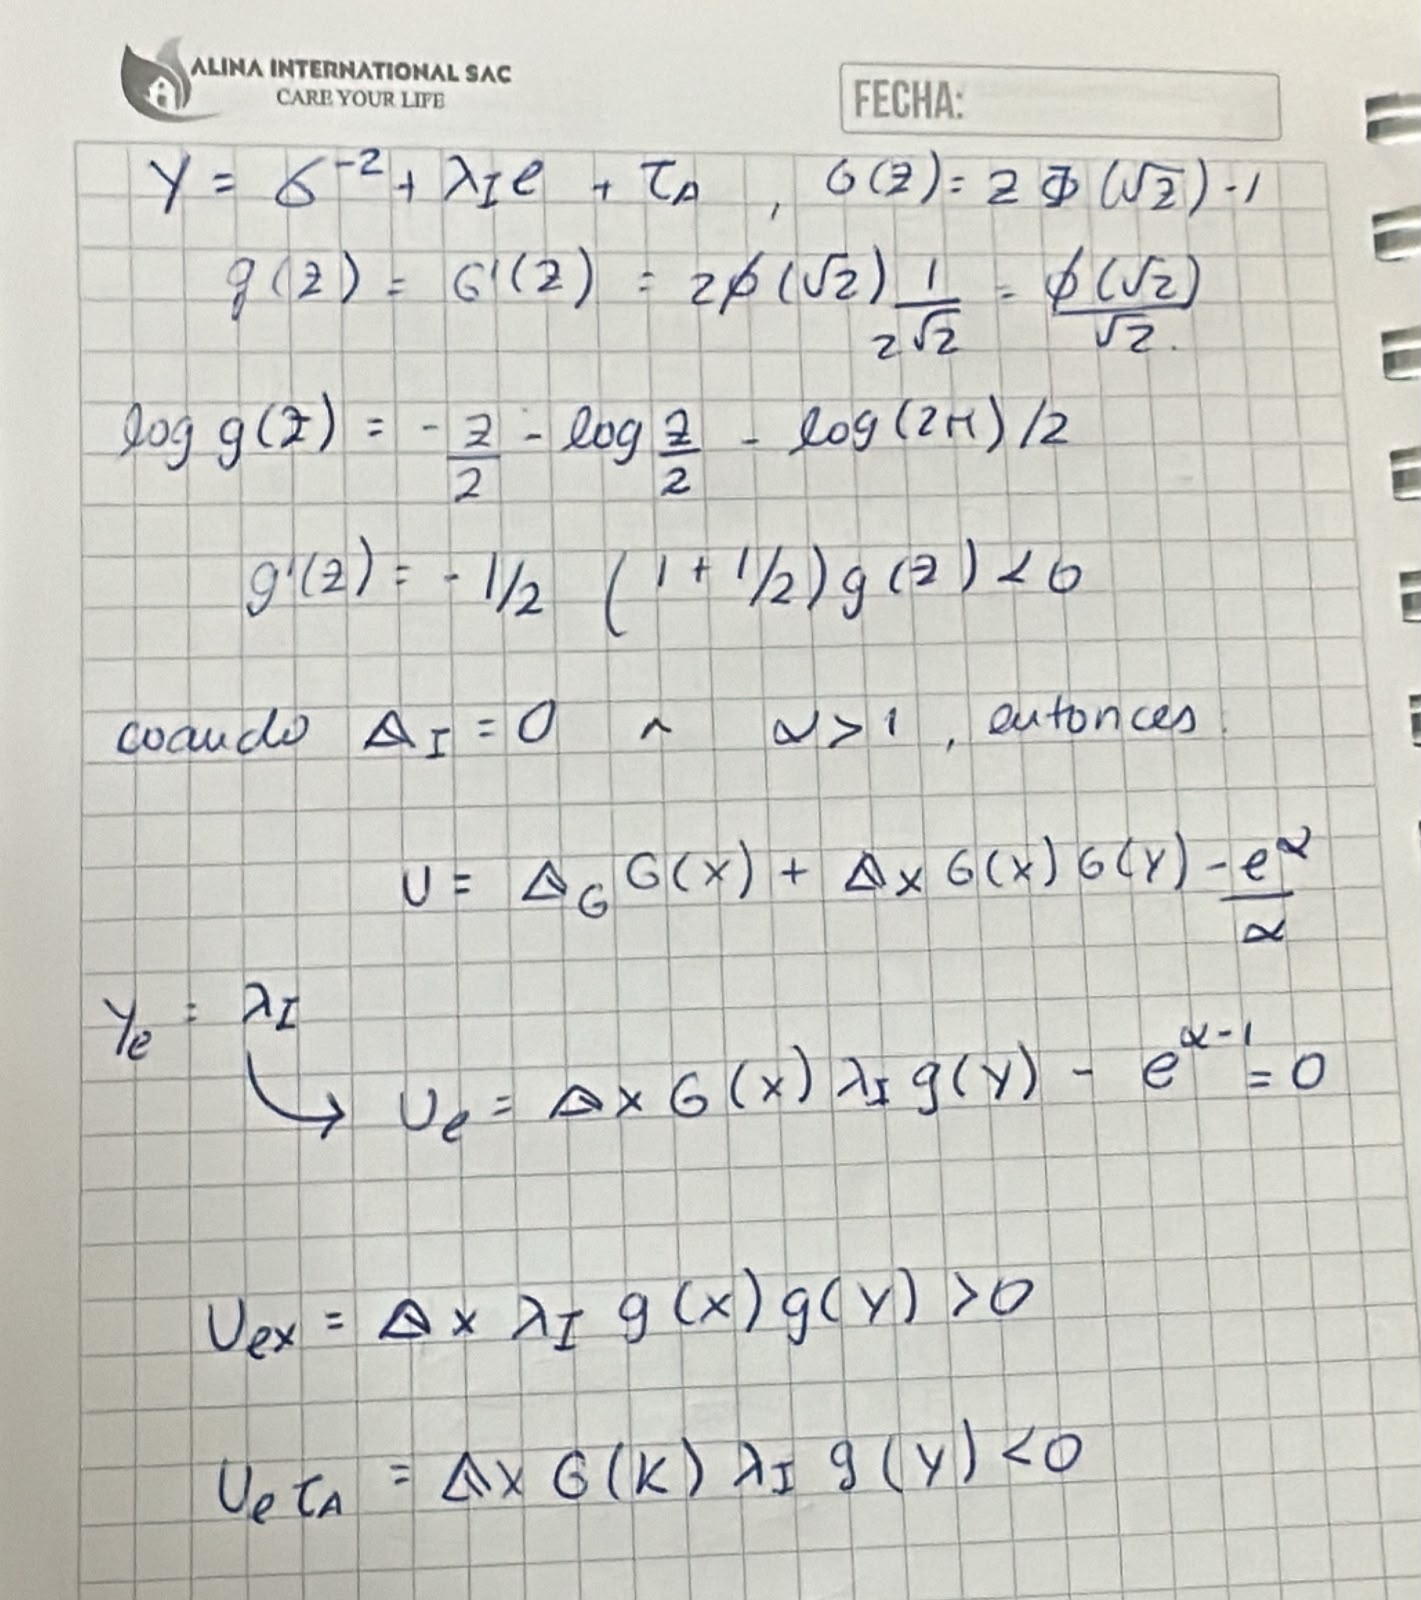
\includegraphics[
        width=\linewidth,
        height=0.56\textheight,
        trim=0 0 0 85,
        clip,
        keepaspectratio
      ]{hand/derivacion-manuscrita-observation-1-david-olano.jpeg}

      \vspace{0.05cm}
      {\scriptsize\color{Muted}Derivación manuscrita de David Olano.}
    \end{column}

    \begin{column}{0.59\textwidth}
      \footnotesize
      {\bfseries Afirmación puesta en duda}\\
      Los signos de Observation 1 podían ocultar supuestos.

      \vspace{0.05cm}
      {\bfseries Qué calculé a mano}\\
      Derivé \(g'(Y)\), la FOC y ambos cross-partials.

      \vspace{0.05cm}
      {\bfseries Qué mostró}\\
      \(U_{eX}>0\) y \(U_{e\tau_A}<0\) bajo los supuestos del modelo, con \(X>0\).

      \vspace{0.05cm}
      {\color{Teal}\bfseries Veredicto}\\
      La IA estaba correcta en el interior, pero incompleta sin las condiciones y la excepción \(X=0\).

      \vspace{0.05cm}
      {\bfseries Bienestar:}
      los signos no implican monotonía en \(\tau_A\). Bajo Assumption 2, los supuestos base y \(\alpha-1\neq 1/4\), los autores obtienen un máximo finito \(\tau_A^*\).
    \end{column}
  \end{columns}
\end{frame}

\end{document}
